\documentclass[12pt]{article}
\usepackage{mathtext}
\usepackage{amsmath}
\usepackage[T2A]{fontenc}
\usepackage[utf8]{inputenc}
\usepackage[russian]{babel}
\usepackage[left=1.5cm, right=1.5cm, top=2cm, bottom=2cm, bindingoffset=0cm]{geometry}
\usepackage{listings}
\usepackage{fancyhdr}
\usepackage{pgfplots}
\pgfplotsset{compat=1.9}



\begin{document}
    \begin{center}
        \textbf{Московский авиационный институт} \\
        \textbf{(Национальный исследовательский университет)}
    \end{center} 
    ~\\
    ~\\
    Институт: «Информационные технологии и прикладная математика» \\
    Кафедра: 805 «Математическая кибернетика»  \\
    Дисциплина: «Численные методы»  
    ~\\
    ~\\
    ~\\
    \begin{center}
        Лабораторная работа №1 \\
        Тема: Решение начально-краевой задачи для дифференциального\\ уравнения 
        параболического типа
    \end{center}
    ~\\
    ~\\
    ~\\
    ~\\
    ~\\
    ~\\
    ~\\
    ~\\
    ~\\
    \begin{flushright}
        Студент: ~~~~~~~~~~~~Хахин Максим~~~~~~\\
        Группа: ~~~~~~~~~~~~~~80-403~~~~~~~~~~~~~~~~~\\
        Преподаватель: ~~~~Иванов И. Э.~~~~~~~\\
        Дата: ~~~~~~~~~~~~~~~~~~~~~~~~~~~~~~~~~~~~~~~~~~~\\
        Оценка: ~~~~~~~~~~~~~~~~~~~~~~~~~~~~~~~~~~~~~~~~\\
    \end{flushright}
    ~\\
    ~\\
    ~\\
    ~\\
    ~\\
    ~\\
    ~\\
    ~\\
    ~\\
    ~\\
    ~\\
    ~\\
    ~\\
    ~\\
    ~\\
    \begin{center}
        Москва, 2021
    \end{center}
    \pagestyle{empty}
    \newpage

    \pagestyle{fancy} 
        \fancyhead{}
        \fancyhead[L]{Хахин Максим}
        \fancyhead[R]{М8О-403Б-18} 
    \fancyfoot{} 
    \begin{enumerate}
        \item \textbf{Задание:}\\
        Используя явную и неявную конечно-разностные схемы, а также схему Кранка - Николсона, решить начально-краевую задачу для дифференциального уравнения параболического типа. Осуществить реализацию трех вариантов аппроксимации граничных условий, содержащих производные: двухточечная аппроксимация с первым порядком, трехточечная аппроксимация со вторым порядком, двухточечная аппроксимация со вторым порядком. В различные моменты времени вычислить погрешность численного решения путем сравнения результатов с приведенным в задании аналитическим решением. Исследовать зависимость погрешности от сеточных параметров.

        \item \textbf{Вариант 9:}\\
        Значния $a = 5,~ b = 3,~ c = 0$
        \begin{figure}[h]
            \center{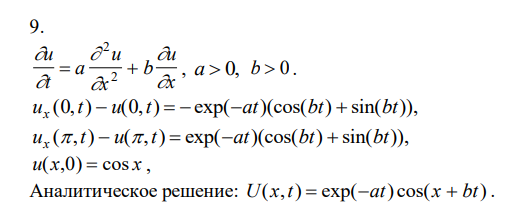
\includegraphics[width=0.5\linewidth]{ 1.png}}
            \label{ris:image}
        \end{figure}\\
        \item \textbf{Теория:}\\
        \begin{center}  \textbf{Разложение ДУ в ряд.} \end{center}
    Диференциальное уравнение с частными производными параболического типа в общем виде записывается следующим образом: 
    $$\frac{\delta u}{\delta t} =a\frac{\delta^2 u}{\delta x^2}+b\frac{\delta u}{\delta x}+cu+f(x,t)$$
    \begin{enumerate}
    \item Для явной разностной схемы.
        \\Воспользуемся методами численного диференциирования и разложим каждый член уравнения имеющий производную в конечную сумму:
        \begin{itemize}
            \item $\frac{\delta u}{\delta t}=\frac{u_i^{k+1}-u_i^{k}}{\tau}$, где  $\tau$ - шаг по временной сетке;
            \item $a\frac{\delta^2 u}{\delta x^2} = a\frac{u_{i-1}^k-2u_{i}^k+u_{i+1}^k}{h^2}$, где  $h$ - шаг по пространственной сетке;
            \item $b\frac{\delta u}{\delta x} = b\frac{u_{i+1}^k-u_{i-1}^k}{2h}$;
            \item $cu = cu_{i}^k$;
        \end{itemize}
        Переппишем исходное уравнение:
        $$\frac{u_i^{k+1}-u_i^{k}}{\tau} =a\frac{u_{i-1}^k-2u_{i}^k+u_{i+1}^k}{h^2}+b\frac{u_{i+1}^k-u_{i-1}^k}{2h}+cu_{i}^k+f(x,t).$$
        Сгруппируем коэффицениты при u с одинаковыми индексами:
        $$u_i^{k+1} = \left(\frac{a}{h^2}-\frac{b}{2h} \right)u_{i-1}^k\tau + \left(c+\frac{1}{\tau}-\frac{2a}{h^2}\right)u_i^k\tau +
        \left(\frac{a}{h^2}+\frac{b}{2h}\right)u_{i+1}^k\tau+f(x,t)\tau.$$
        Непосредственно из этого уравнения находится значение функции на временном уровне k+1.
    \item Для не явной разностной схемы.
        \\Воспользуемся методами численного диференциирования и разложим каждый член уравнения имеющий производную в конечную сумму:
        \begin{itemize}
            \item $\frac{\delta u}{\delta t}=\frac{u_i^{k+1}-u_i^{k}}{\tau}$, где  $\tau$ - шаг по временной сетке;
            \item $a\frac{\delta^2 u}{\delta x^2} = a\frac{u_{i-1}^{k+1}-2u_{i}^{k+1}+u_{i+1}^{k+1}}{h^2}$, где  $h$ - шаг по пространственной сетке;
            \item $b\frac{\delta u}{\delta x} = b\frac{u_{i+1}^{k+1}-u_{i-1}^{k+1}}{2h}$;
            \item $cu = cu_{i}^{k+1}$;
        \end{itemize}
        Переппишем исходное уравнение:
        $$\frac{u_i^{k+1}-u_i^{k}}{\tau} =a\frac{u_{i-1}^{k+1}-2u_{i}^{k+1}+u_{i+1}^{k+1}}{h^2}+b\frac{u_{i+1}^{k+1}-u_{i-1}^{k+1}}{2h}+cu_{i}^{k+1}+f(x,t).$$
        Сгруппируем коэффицениты при u с одинаковыми индексами:
        $$u_i^{k}+f(x,t)\tau = \left(\frac{b}{2h}-\frac{a}{h^2} \right)u_{i-1}^{k+1}\tau + \left(\frac{1}{\tau}+\frac{2a}{h^2}-c\right)u_i^{k+1}\tau -
        \left(\frac{a}{h^2}+\frac{b}{2h}\right)u_{i+1}^{k+1}\tau.$$
        Для нахождения значений функции u на уровне k+1 необходимо решить систему уравнеий:
        \begin{equation*}
            \begin{cases}
                i=1;\:\:\: ...
                \\
                i=\overline{2,N-1};\:\:\:Au_{i-1}^{k+1} + Bu_i^{k+1} +Cu_{i+1}^{k+1}=d_i
                \\
                i=N;\:\:\: ...
            \end{cases}
        \end{equation*}
        где $A = \left(\frac{b}{2h}-\frac{a}{h^2} \right)\tau$, $B = \left(\frac{1}{\tau}+\frac{2a}{h^2}-c\right)\tau$, $C = -\left(\frac{a}{h^2}+\frac{b}{2h}\right)\tau$, 
        $d = u_i^{k}+f(x,t)\tau$.\\
        Формирование уравнеий при i=1 и i=N рассмотрим в разделе посвященном краевые условия.
    \end{enumerate}
    \textbf{Примечание.}
    \emph{Во всех формулах приведенных выше рассматривается $i \in [2,N-1]$, где N - количекство узлов в сетке по координате x.}

    \begin{center}  \textbf{Краевые условия.} \end{center}
    Краевые условия могут принимать вид:
    \begin{enumerate}
        \item Условия первого рода:
            \begin{equation*}
                \begin{cases}
                    \beta u(0,x) = \phi_l(t)
                    \\
                    \delta u(l,x) = \phi_r(t)
                \end{cases}
            \end{equation*}
            В таком случае $u_1^{k+1}$ и $u_N^{k+1}$ находятся по формуле:
            \begin{itemize}
                \item Для явной разностной схемы\\
                $u_1^{k+1}=\frac{\phi_l(t)}{\beta}$, $u_N^{k+1}=\frac{\phi_r(t)}{\delta}$.
                \item Для не явной разностной схемы\\
                \begin{equation*}
                    \begin{cases}
                        i=1;\:\:\: \beta u_1^{k+1} +0u_{2}^{k+1}=\phi_l(t)
                        \\
                        i=\overline{2,N-1};\:\:\:Au_{i-1}^{k+1} + Bu_i^{k+1} +Cu_{i+1}^{k+1}=d_i
                        \\
                        i=N;\:\:\: 0u_{N-1}^{k+1} + \delta u_N^{k+1} = \phi_r(t)
                    \end{cases},
                \end{equation*}
            \end{itemize}

        \item Условия второго рода:
            \begin{equation*}
                \begin{cases}
                    \frac{\delta u}{\delta x}(0,x) = \frac{\phi_l(t)}{\alpha}
                    \\
                    \frac{\delta u}{\delta x}(l,x) = \frac{\phi_r(t)}{\gamma}
                \end{cases}
                \Leftrightarrow
                \begin{cases}
                    \frac{u_{2}^{k+1}-u_{1}^{k+1}}{h}(0,x) = \frac{\phi_l(t)}{\alpha}
                    \\
                    \frac{u_{N}^{k+1}-u_{N-1}^{k+1}}{h}(l,x) = \frac{\phi_r(t)}{\gamma}
                \end{cases}
            \end{equation*}
            В таком случае $u_1^{k+1}$ и $u_N^{k+1}$ находятся по формуле:
            \begin{itemize}
                \item Для явной разностной схемы\\
                $u_1^{k+1}=u_2^{k+1}-h\frac{\phi_l(t)}{\alpha}$, $u_N^{k+1}=u_{N-1}^{k+1}+h\frac{\phi_r(t)}{\gamma}$.
                \item Для не явной разностной схемы\\
                \begin{equation*}
                    \begin{cases}
                        i=1;\:\:\: -\frac{\alpha}{h}u_1^{k+1} +\frac{\alpha}{h}u_{2}^{k+1}=\phi_l(t)
                        \\
                        i=\overline{2,N-1};\:\:\:Au_{i-1}^{k+1} + Bu_i^{k+1} +Cu_{i+1}^{k+1}=d_i
                        \\
                        i=N;\:\:\: -\frac{\gamma}{h}u_{N-1}^{k+1} +\frac{\gamma}{h}u_{N}^{k+1}=\phi_r(t)
                    \end{cases},
                \end{equation*}
            \end{itemize}
        
        \item Условия третьего рода:
            \begin{equation*}
                \begin{cases}
                    \alpha\frac{\delta u}{\delta x}(0,x) + \beta u(0,x)= \phi_l(t)
                    \\
                    \gamma\frac{\delta u}{\delta x}(l,x) + \delta u(l,x)= \phi_r(t)
                \end{cases}
                \Leftrightarrow
                \begin{cases}
                    \alpha\frac{u_{2}^{k+1}-u_{1}^{k+1}}{h}(0,x) + \beta u_{1}^{k+1} = \phi_l(t)
                    \\
                    \gamma\frac{u_{N}^{k+1}-u_{N-1}^{k+1}}{h}(l,x) + \delta u_{N}^{k+1}= \phi_r(t)
                \end{cases}
            \end{equation*}
            В таком случае $u_1^{k+1}$ и $u_N^{k+1}$ находятся по формуле:
            \begin{itemize}
                \item Для явной разностной схемы\\
                $u_1^{k+1}=\frac{\phi_l(t)-\frac{\alpha}{h}u_2^{k+1}}{\beta-\frac{\alpha}{h}}$, 
                $u_N^{k+1}=\frac{\phi_r(t)+\frac{\gamma}{h}n_{N-1}^{k+1}}{\delta+\frac{\gamma}{h}}$.
                \item Для не явной разностной схемы\\
                \begin{equation*}
                    \begin{cases}
                        i=1;\:\:\: \left(\beta-\frac{\alpha}{h}\right)u_1^{k+1} +\frac{\alpha}{h}u_{2}^{k+1}=\phi_l(t)
                        \\
                        i=\overline{2,N-1};\:\:\:Au_{i-1}^{k+1} + Bu_i^{k+1} +Cu_{i+1}^{k+1}=d_i
                        \\
                        i=N;\:\:\: -\frac{\gamma}{h}u_{N-1}^{k+1} + \left(\delta+\frac{\gamma}{h}\right)u_N^{k+1} =\phi_r(t)
                    \end{cases},
                \end{equation*}
            \end{itemize}
    \end{enumerate}
    \textbf{Примечание.}
    \emph{в разборе приведена апроксимация краевых условий с производной по 2 точкам с 1 порядком точности. Так же можно апроксимировать краевое 
    условие по 3 точкам с точностью 2 и по 2 точкам с точностью 2.}
        \item \textbf{Код:}\\
        \begin{lstlisting}[language=C]
            \\Define the initial boundary conditions


double phi(double x)
{
    return -exp(-1*x)*(cos(1*x)+sin(1*x));
} 
double phil(double x)
{
    return exp(-1*x)*(cos(1*x)+sin(1*x));
} 
double ksi(double x)
{
    return cos(x);
}
double f(double x, double t)
{
    return 0;
}


            \\explicit


void get_first_layer_explicit(int pr, int k, int N, double l,
 double T, double *args1, double *args2, matrix *grid,
  double(*phi)(double), double(*phil)(double), double(*ksi)(double),
   double(*f)(double, double))
{
    double tau = T/k, h = l/(N-1), mu = args1[1]*tau/(2*h);
    double b0, c0, bN, aN, d0, dN;

    for(int i=0; i<N; i++)
        *get_element(grid, 0, i) = ksi(i*h);
    
    for(int i=1; i<k; i++)
        for(int j=1; j<N-1; j++)
            *get_element(grid, i, j) = *get_element(grid, i-1, j+1)*
            (T + mu)+(*get_element(grid, i-1, j)*(1-2*T+ tau*args1[2]))+
            (*get_element(grid, i-1, j-1)*(T-mu));
    
    switch (pr)
    {
    case 1:
        for(int i=1; i<k; i++)
        {
            *get_element(grid, i, 0) = (*get_element(grid, i, 1)*
            (-args2[0]/h)+phi(tau*k))/(args2[1] - args2[0] / h);
            *get_element(grid, i, N-1) = (*get_element(grid, i, N-2)*
            (args2[2]/h)+phil(tau*k))/(args2[3] + args2[2] / h);
        }
        break;
    case 2:
        for(int i=1; i<k; i++)
        {
            *get_element(grid, i, 0) = ((*get_element(grid, i, 1)*
            4-*get_element(grid, i, 2))*(-args2[0]/(2*h))+phi(tau*k))/
            (args2[1] - 3*args2[0]/(2*h));
            *get_element(grid, i, N-1) = ((*get_element(grid, i, N-3)-
            *get_element(grid, i, N-2)*4)*(-args2[2]/(2*h))+phil(tau*k))/
            (args2[3] + 3*args2[2]/(2*h));
        }
        break;
    case 3:
        b0 = 2*args1[0]/h + h/tau - h*args1[2] - args2[1]/args2[0]*
        (2*args1[0] - args1[1]*h);
        c0 = -2*args1[0]/h;
        bN = 2*args1[0]/h + h/tau - h*args1[2] + args2[3]/args2[2]*
        (2*args1[0] + args1[1]*h);
        aN = -2*args1[0]/h;
        for(int i=1; i<k; i++)
        {
            d0 = h/tau * (*get_element(grid, i-1, 0)) - phi(tau*(k + 1)) *
            (2*args1[0] - args1[1]*h) / args2[0];
            dN = h/tau * (*get_element(grid, i-1, N-1))+ phil(tau*(k + 1)) *
            (2*args1[0] - args1[1]*h) / args2[2];
            *get_element(grid, i, 0) = (d0 - c0 * 
            (*get_element(grid, i, 1))) / b0;
            *get_element(grid, i, N-1) = (dN - aN * 
            (*get_element(grid, i, N-2))) / bN;
        }
        break;
    }
}


            \implicit


void get_first_layer_implicit(int pr, int k, int N, double l, double T,
 double *args1, double *args2, matrix *grid, double(*phi)(double),
  double(*phil)(double), double(*ksi)(double), double(*f)(double, double))
{
    double tau = T/k, h = l/(N-1);
    matrix system = create_matrix(N, N);
    matrix D = create_matrix(1,N);
    
    for(int i=0; i<N; i++)
        *get_element(grid, 0, i) = ksi(i*h);
    
    for (int i=1; i<N-1; i++)
    {
        *get_element(&system, i, i-1) = args1[0]*tau/pow(h,2)-
        args1[1]*tau/(2*h);
        *get_element(&system, i, i) = -2*args1[0]*tau/pow(h,2)+
        args1[2]*tau-1;
        *get_element(&system, i, i+1) = args1[0]*tau/pow(h,2)+
        args1[1]*tau/(2*h);
    }
    
    switch (pr)
    {
    case 1:
        *get_element(&system, 0, 0) = args2[1] - args2[0] / h;
        *get_element(&system, 0, 1) = args2[0] / h;
        *get_element(&system, N-1, N-2) = - args2[2] / h;
        *get_element(&system, N-1, N-1) = args2[3] + args2[2] / h;
        break;
    case 2:
        *get_element(&system, 0, 0) = args2[1] - 3*args2[0]/ h/ 2;
        *get_element(&system, 0, 1) = 2 * args2[0]/h;
        *get_element(&system, 0, 2) = - args2[0] / h /2;
        *get_element(&system, N-1, N-3) = args2[2] / h /2;
        *get_element(&system, N-1, N-2) = -2 * args2[2]/h;
        *get_element(&system, N-1, N-1) = args2[3] + 3*args2[2]/ h/ 2;
        break;
    case 3:
        *get_element(&system, 0, 0) = 2 * args1[0] / h + h / tau - h * 
        args1[2] - args2[1] / args2[0] * (2 * args1[0] - args1[1] * h);
        *get_element(&system, 0, 1) = -2 * args1[0] / h;
        *get_element(&system, N-1, N-2) = -2 * args1[0] / h;
        *get_element(&system, N-1, N-1) = 2 * args1[0] / h + h / tau - 
        h * args1[2] + args2[3] / args2[2] * (2 * args1[0] + args1[1] * h);
        break;
    }
    for(int i=1; i<k; i++)
    {
        for(int j=1; j<N-1; j++)
            *get_element(&D, 0, j) = -(*get_element(grid, i-1, j));
        switch (pr)
        {
        case 1:
            *get_element(&D, 0, 0) = phi(i*tau);
            *get_element(&D, 0, N-1) = phil(i*tau);
            insert_matrix_line(grid, run_method(system, D, N), i);
            break;
        case 2:
            *get_element(&D, 0, 0) = phi(i*tau);
            *get_element(&D, 0, N-1) = phil(i*tau);
            insert_matrix_line(grid, LU_method(system, D, N), i);
            break;
        case 3:
            *get_element(&D, 0, 0) = h / tau * (*get_element(grid, i-1, 0))-
            phi(tau*i) * (2 * args1[0] - args1[1] * h) / args2[0];
            *get_element(&D, 0, N-1) = h/tau*(*get_element(grid, i-1, N-1))+
            phil(tau*i) * (2 * args1[0] + args1[1] * h) / args2[2];
            insert_matrix_line(grid, run_method(system, D, N), i);
            break;
        }
    }
    //destroy_matrix(&system); destroy_matrix(&D); destroy_matrix(&tmp);
}
        

            \\CrankNicolson


void get_first_layer_CrankNicolson(int pr, int k, int N, double sgm, 
double l, double T,double *args1, double *args2, matrix *grid, 
double(*phi)(double), double(*phil)(double),
double(*ksi)(double), double(*f)(double, double))
{
    matrix grid1 = create_matrix(k,N);
    matrix grid2 = create_matrix(k,N);
    get_first_layer_explicit(pr, k, N, l, T, args1, args2, 
    &grid1, phi, phil, ksi, f);
    get_first_layer_implicit(pr, k, N, l, T, args1, args2, 
    &grid2, phi, phil, ksi, f);
    printf("y");
    for (int i=0; i<k; i++)
        for (int j=0; j<N; j++)
            *get_element(grid, i, j) = *get_element(&grid1, i, j)*(1-sgm)+
            *get_element(&grid2, i, j)*sgm;
}

        \end{lstlisting}
        \item \textbf{Результат:}\\
        Явный метод сетка 1000*100: 
        \begin{figure}[h]
            \center{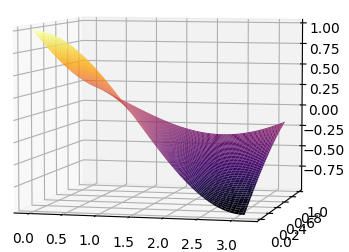
\includegraphics[width=0.3\linewidth]{ 2.2.png}}
            \label{ris:image}
        \end{figure}\\
        \newpage    
        Ошибка : 0.0857908889653587
        \\Явный метод сетка 2000*200: 
        \begin{figure}[h]
            \center{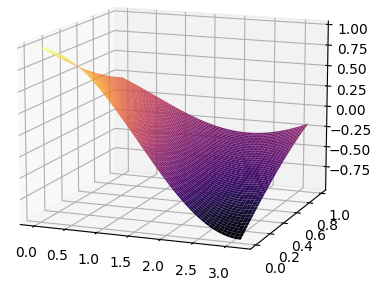
\includegraphics[width=0.3\linewidth]{ 2.1.png}}
            \label{ris:image}
        \end{figure}\\
        Ошибка: 0.0792584889653587 
        \\Явный метод сетка 4000*400: 
        \begin{figure}[h]
            \center{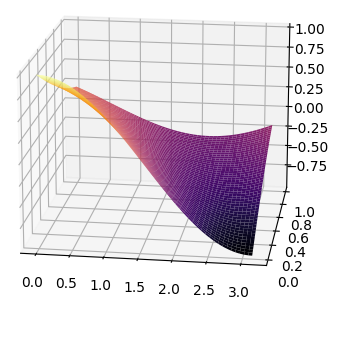
\includegraphics[width=0.3\linewidth]{ 2.png}}
            \label{ris:image}
        \end{figure}\\
        
        Ошибка : 0.0565016889653587
        \\  Ошибка с разным шагом по времени:
        \begin{figure}[h]
            \center{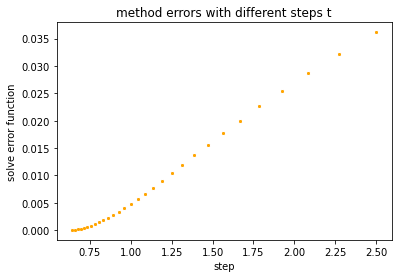
\includegraphics[width=0.5\linewidth]{ 3.png}}
            \label{ris:image}
        \end{figure}\\
        \newpage
        Ошибка с разным шагом по пространству:
        \begin{figure}[h]
            \center{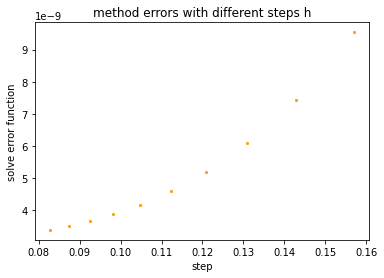
\includegraphics[width=0.5\linewidth]{ 4.png}}
            \label{ris:image}
        \end{figure}\\
        
        Неявный метод сетка 1000*100: 
        \begin{figure}[!h]
            \center{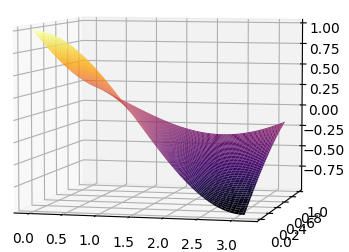
\includegraphics[width=0.3\linewidth]{ 2.2.png}}
            \label{ris:image}
        \end{figure}\\
  \newpage
        Ошибка : 0.007134110346412981
        \\Неявный метод сетка 2000*200: 
        \begin{figure}[h]
            \center{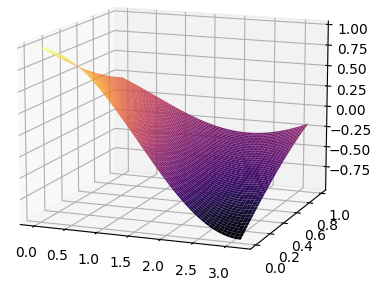
\includegraphics[width=0.3\linewidth]{ 2.1.png}}
            \label{ris:image}
        \end{figure}\\
        Ошибка: 0.0070211103464130065 
        \\Неявный метод сетка 4000*400: 
        \begin{figure}[h]
            \center{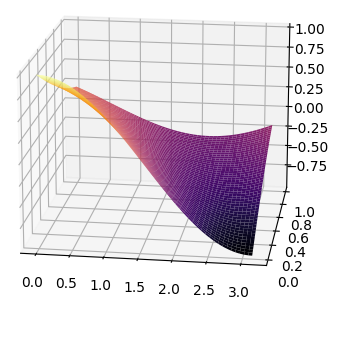
\includegraphics[width=0.3\linewidth]{ 2.png}}
            \label{ris:image}
        \end{figure}\\
        
        Ошибка : 0.0069961103464129815
        \\  Ошибка с разным шагом по времени:
        \begin{figure}[h]
            \center{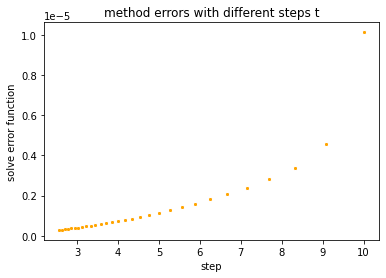
\includegraphics[width=0.5\linewidth]{ 5.png}}
            \label{ris:image}
        \end{figure}\\
        \newpage
        Ошибка с разным шагом по пространству:
        \begin{figure}[h]
            \center{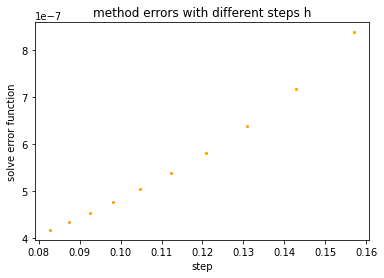
\includegraphics[width=0.5\linewidth]{ 6.png}}
            \label{ris:image}
        \end{figure}\\

        КН метод сетка 1000*100: 
        \begin{figure}[!h]
            \center{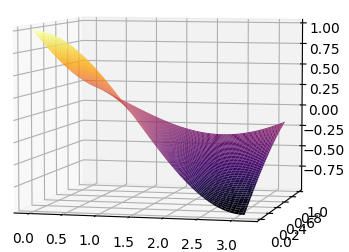
\includegraphics[width=0.3\linewidth]{ 2.2.png}}
            \label{ris:image}
        \end{figure}\\
        Ошибка : 0.0000222043352098354
        \\КН метод сетка 2000*200: 
        \begin{figure}[!h]
            \center{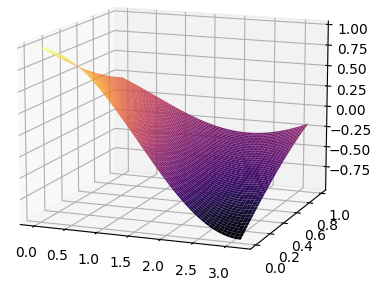
\includegraphics[width=0.3\linewidth]{ 2.1.png}}
            \label{ris:image}
        \end{figure}\\
        
        Ошибка: 0.00001963083520983543
        \newpage
        \\КН метод сетка 4000*400: 
        \begin{figure}[h]
            \center{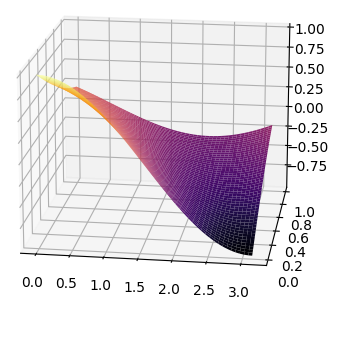
\includegraphics[width=0.3\linewidth]{ 2.png}}
            \label{ris:image}
        \end{figure}\\
        
        Ошибка : 0.000011319135209835429
        \\  Ошибка с разным шагом по времени:
        \begin{figure}[h]
            \center{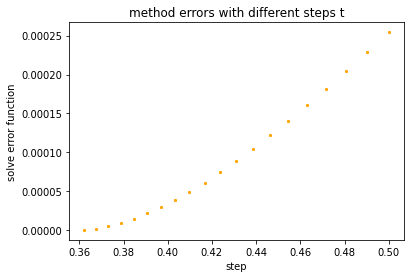
\includegraphics[width=0.5\linewidth]{ 7.png}}
            \label{ris:image}
        \end{figure}\\

        Ошибка с разным шагом по пространству:
        \begin{figure}[h]
            \center{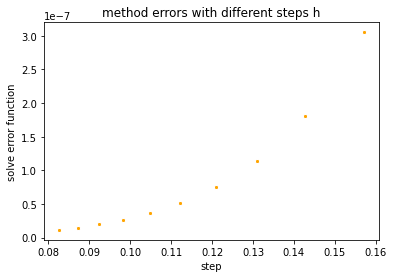
\includegraphics[width=0.5\linewidth]{ 8.png}}
            \label{ris:image}
        \end{figure}\\
\newpage

        \item \textbf{Вывод:}\\
        В результате выполнения лабораторной работы были освоены 3 конечно-разностные схемы для решения начально-краевой задачи для дифференциального уравнения параболического типа : явная конечно-разностная схема, неявная конечно-разностная схема и схема Кранка - Николсона.
\\Были построены графики ошибок, на которых показано падение ошибки при росте числа разбиений по пространству и времени.

        
    \end{enumerate}
\end{document}